\documentclass[aspectratio=169]{beamer}
% For best font rendering with XeLaTeX/LuaLaTeX
\usepackage{fontspec}
\usepackage{unicode-math}
\usepackage{tikz}
\usepackage{colortbl}
\usepackage{amsmath}
\usepackage{amssymb}
\usepackage{graphicx}
\usepackage{hyperref}
\usepackage{algorithm}
\usepackage{algpseudocode}
\usepackage{booktabs}
\usepackage{multirow}
\usepackage{xcolor}
\usepackage{listings}
\usepackage{biblatex}

% TikZ libraries
\usetikzlibrary{arrows,automata,positioning,shapes,calc,decorations.pathmorphing,patterns,math}

% Beamer theme
\usetheme{metropolis}

% Title page info
\title{Probabilistic Algorithms: What, Why, and How}
\subtitle{A Deep Dive into Randomness in Computing}
\author{Sailesh Dahal}
\institute{Kathmandu University}
\date{\today}

% Bibliography
\addbibresource{refs.bib}

% Listings configuration
\lstset{
    language=Python,
    basicstyle=\ttfamily\small,
    breaklines=true,
    frame=single,
    numbers=left,
    numberstyle=\tiny,
    keywordstyle=\color{blue},
    commentstyle=\color{green!60!black},
    stringstyle=\color{red},
    showstringspaces=false
}

\begin{document}

\begin{frame}
  \begin{tikzpicture}[remember picture,overlay]
    \node[anchor=south east, xshift=-5mm, yshift=5mm] at (current page.south east) {
      
\includegraphics[width=2cm]{../assets/ku_logo.png}
    };
  \end{tikzpicture}
  \titlepage
\end{frame}

% Outline frame
\begin{frame}{Outline}
  \tableofcontents
\end{frame}

% What are Probabilistic Algorithms?
\section{What are Probabilistic Algorithms?}
\begin{frame}{What is a Probabilistic Algorithm?}
  \begin{block}{Definition}
    An algorithm that makes random choices during execution to influence its behavior or output.
  \end{block}

  \begin{itemize}
    \item Output or performance may vary on different runs
    \item Two main types: Las Vegas (always correct, time varies), Monte Carlo (time fixed, may err)
  \end{itemize}
\end{frame}

\begin{frame}{Types of Probabilistic Algorithms}
  \begin{itemize}
    \item \textbf{Las Vegas:} Always correct, random running time

    \item \textbf{Monte Carlo:} Fixed running time, may give incorrect result with small probability

    \item \textbf{Example:} Randomized Quicksort (Las Vegas)

    \item \textbf{Example:} Primality testing (Monte Carlo)
  \end{itemize}
\end{frame}

% Why use Probabilistic Algorithms?
\section{Why Probabilistic Algorithms?}
\begin{frame}{Why Randomness?}
  \begin{block}{Motivation}
    \begin{itemize}
      \item Simpler algorithms

      \item Better expected performance

      \item Avoid worst-case scenarios

      \item Useful for large-scale and distributed systems
    \end{itemize}
  \end{block}
\end{frame}

\begin{frame}{Real-World Motivation}
  \begin{itemize}
    \item Web search (PageRank)

    \item Load balancing (power of two choices)

    \item Hashing (universal hash functions)

    \item Primality testing (Miller-Rabin)
  \end{itemize}
\end{frame}

% How do Probabilistic Algorithms work?
\section{How do Probabilistic Algorithms Work?}
\begin{frame}{How: Randomization in Algorithms}
  \begin{block}{Key Idea}
    Use random choices to influence the algorithm's path or output.
  \end{block}

  \begin{itemize}
    \item Random pivot in Quicksort

    \item Random walks in graphs

    \item Random sampling
  \end{itemize}
\end{frame}

% Example: Randomized Quicksort
\section{Example: Randomized Quicksort}

% New slide: QuickSort vs Randomized QuickSort steps
\begin{frame}{QuickSort vs Randomized QuickSort}
\textbf{QuickSort:}
\begin{enumerate}
  \item Pick a pivot element from the array
  \item Split array into 3 subarrays: those smaller than pivot, those larger than pivot, and the pivot itself
  \item Recursively sort the subarrays, and concatenate them
\end{enumerate}
  \vspace{1em}
  \textbf{Randomized QuickSort:}
  \begin{enumerate}
    \item Pick a pivot element \textbf{uniformly at random} from the array
    \item Split array into 3 subarrays: those smaller than pivot, those larger than pivot, and the pivot itself
    \item Recursively sort the subarrays, and concatenate them
  \end{enumerate}
  \end{frame}

% New slide: Worst-case for QuickSort
\begin{frame}{Example: Randomized Quicksort}
  \textbf{Recall:} QuickSort can take $\Omega(n^2)$ time to sort an array of size $n$.
\end{frame}

% New slide: Theorem and expectation for Randomized QuickSort
\begin{frame}{Randomized QuickSort: Expected Runtime}
\textbf{Theorem}
\begin{block}{}
  Randomized QuickSort sorts a given array of length $n$ in $O(n \log n)$ expected time.
\end{block}
  \vspace{1em}
  \textbf{Note:} On every input, randomized QuickSort takes $O(n \log n)$ time in expectation. On every input, it may take $\Omega(n^2)$ time with some small probability.
\end{frame}

\section{Example: Randomized Quicksort}

% New slide: QuickSort vs Randomized QuickSort steps
\begin{frame}{QuickSort vs Randomized QuickSort}
  \textbf{QuickSort:}
  \begin{enumerate}
    \item Pick a pivot element from the array \parencite{10.1093/comjnl/5.1.10}
    \item Split array into 3 subarrays: those smaller than pivot, those larger than pivot, and the pivot itself
    \item Recursively sort the subarrays, and concatenate them
  \end{enumerate}
  \vspace{1em}
  \textbf{Randomized QuickSort:}
  \begin{enumerate}
    \item Pick a pivot element \textbf{uniformly at random} from the array \parencite{motwani1995randomized}
    \item Split array into 3 subarrays: those smaller than pivot, those larger than pivot, and the pivot itself
    \item Recursively sort the subarrays, and concatenate them
  \end{enumerate}
\end{frame}

% New slide: Worst-case for QuickSort
\begin{frame}{Example: Randomized Quicksort}
  \textbf{Recall:} QuickSort can take $\Omega(n^2)$ time to sort an array of size $n$ \parencite{359631}
\end{frame}

% New slide: Theorem and expectation for Randomized QuickSort
\begin{frame}{Randomized QuickSort: Expected Runtime}
  \textbf{Theorem}
  \begin{block}{}
    Randomized QuickSort sorts a given array of length $n$ in $O(n \log n)$ expected time. \parencite{journals/acta/Sedgewick77}
  \end{block}
  \vspace{1em}
  \textbf{Note:} On every input, randomized QuickSort takes $O(n \log n)$ time in expectation. On every input, it may take $\Omega(n^2)$ time with some small probability.
\end{frame}

\subsection{Step-by-Step Execution}
\begin{frame}{Randomized Quicksort: Step 1 (Initial Array)}
  % Use columns for top-aligned split layout
  \begin{columns}[t]
    \column{0.6\textwidth}
    Consider the array:
    \[
      \renewcommand{\arraystretch}{1.5}
      \begin{array}{|c|c|c|c|c|c|c|c|}
        \hline
        15 & 3 & 1 & 10 & 9 & 0 & 6 & 4 \\
        \hline
      \end{array}
    \]
  \end{columns}
\end{frame}

\begin{frame}{Randomized Quicksort: Step 1.1 (Pivot Chosen)}
  % Use columns for top-aligned split layout
  \begin{columns}[t]
    \column{0.6\textwidth}
    Suppose the random pivot chosen is \textcolor{red}{10} (at index 3):
    \[
      \renewcommand{\arraystretch}{1.5}
      \begin{array}{|c|c|c|c|c|c|c|c|}
        \hline
        15 & 3 & 1 & \cellcolor{red!20}\textcolor{red}{10} & 9 & 0 & 6 & 4 \\
        \hline
      \end{array}
    \]
    \pause
    \column{0.38\textwidth}
    \begin{minipage}[t]{\linewidth}
      \vspace{0pt}
      \begin{center}
        \begin{tikzpicture}[
          scale=0.85,
          transform shape,
          level distance=1.5cm,
          level 1/.style={sibling distance=3.0cm},
          level 2/.style={sibling distance=2.0cm},
          level 3/.style={sibling distance=1.2cm},
          every node/.style={font=\tiny}
        ]
          \node[circle, draw, fill=green!20, minimum size=1cm, align=center] (root) {
            \textbf{A[0,7]} \\
            10
          };
        \end{tikzpicture}
      \end{center}
    \end{minipage}
  \end{columns}
\end{frame}
% Step 2: Partitioning around 10
\begin{frame}{Randomized Quicksort: Step 2 (Partitioning Around Pivot 10)}
  % Use columns for top-aligned split layout
  \begin{columns}[t]
    \column{0.6\textwidth}
    After selecting pivot 10, we partition the array:
    \begin{itemize}
      \item \textcolor{green!60!black}{Left:} 4, 3, 1, 9, 0, 6 (elements before pivot position)
      \item \textcolor{red}{Middle:} 10 (pivot)
      \item \textcolor{blue}{Right:} 15 (element after pivot position)
    \end{itemize}
    \pause
    After partitioning:
    \[
      \renewcommand{\arraystretch}{1.5}
      \begin{array}{|c|c|c|c|c|c|c|c|}
        \hline
        \cellcolor{green!20}\textcolor{green!60!black}{4} & \cellcolor{green!20}\textcolor{green!60!black}{3} & \cellcolor{green!20}\textcolor{green!60!black}{1} & \cellcolor{green!20}\textcolor{green!60!black}{9} & \cellcolor{green!20}\textcolor{green!60!black}{0} & \cellcolor{green!20}\textcolor{green!60!black}{6} & \cellcolor{red!20}\textcolor{red}{10} & 15 \\
        \hline
      \end{array}
    \]
    \pause
    \column{0.38\textwidth}
    \begin{minipage}[t]{\linewidth}
      \vspace{0pt}
      \begin{center}
        \begin{tikzpicture}[
          scale=0.85,
          transform shape,
          level distance=1.5cm,
          level 1/.style={sibling distance=3.0cm},
          level 2/.style={sibling distance=2.0cm},
          level 3/.style={sibling distance=1.2cm},
          every node/.style={font=\tiny}
        ]
          % Root node
          \node[circle, draw, fill=green!20, minimum size=1cm, align=center] (root) {
            \textbf{A[0,7]} \\
            10
          }
          % Left child
          child {node[circle, draw, fill=green!20, minimum size=1cm, align=center] {
                  \textbf{A[0,5]}
                }}
          % Right child
          child {node[circle, draw, fill=white, minimum size=1cm, align=center] {
                  \textbf{A[7,7]}
                }};
        \end{tikzpicture}
      \end{center}
    \end{minipage}
  \end{columns}
\end{frame}

% Step 3: Recurse Left [A[0,5]], Pivot 4
\begin{frame}{Randomized Quicksort: Step 3 (Recurse Left [A[0,5]], Pivot 4)}
  % Use columns for top-aligned split layout
  \begin{columns}[t]
    \column{0.6\textwidth}
    Recurse on the left subarray:
    \\[0.5em]
    Let's choose a random pivot, say 4.
    \[
      \renewcommand{\arraystretch}{1.5}
      \begin{array}{|c|c|c|c|c|c|}
        \hline
        \cellcolor{red!20}\textcolor{red}{4} & 3 & 1 & 9 & 0 & 6 \\
        \hline
      \end{array}
    \]
    \pause
    \column{0.38\textwidth}
    \begin{minipage}[t]{\linewidth}
      \vspace{0pt}
      \begin{center}
        \begin{tikzpicture}[
          scale=0.85,
          transform shape,
          level distance=1.5cm,
          level 1/.style={sibling distance=3.0cm},
          level 2/.style={sibling distance=2.0cm},
          level 3/.style={sibling distance=1.2cm},
          every node/.style={font=\tiny}
        ]
          % Root node
          \node[circle, draw, fill=green!20, minimum size=1cm, align=center] (root) {
            \textbf{A[0,7]} \\
            10
          }
          % Left child
          child {node[circle, draw, fill=green!20, minimum size=1cm, align=center] {
                  \textbf{A[0,5]} \\
                  4
                }}
          % Right child
          child {node[circle, draw, fill=white, minimum size=1cm, align=center] {
                  \textbf{A[7,7]}
                }};
        \end{tikzpicture}
      \end{center}
    \end{minipage}
  \end{columns}
\end{frame}

% Step 3.1: Partition Left [A[0,5]] Around 4
\begin{frame}{Randomized Quicksort: Step 3.1 (Partition Left [A[0,5]] Around 4)}
  % Use columns for top-aligned split layout
  \begin{columns}[t]
    \column{0.6\textwidth}
    After partitioning the left subarray:
    \[
      \renewcommand{\arraystretch}{1.5}
      \begin{array}{|c|c|c|c|c|c|}
        \hline
        \cellcolor{green!20}\textcolor{green!60!black}{0} & \cellcolor{green!20}\textcolor{green!60!black}{3} & \cellcolor{green!20}\textcolor{green!60!black}{1} & \cellcolor{red!20}\textcolor{red}{4} & 9 & 6 \\
        \hline
      \end{array}
    \]
    Partition:
    \begin{itemize}
      \item \textcolor{green!60!black}{Left:} 0, 3, 1 (elements before pivot)
      \item \textcolor{red}{Middle:} 4 (pivot)
      \item \textcolor{blue}{Right:} 9, 6 (elements after pivot)
    \end{itemize}
    \pause
    \column{0.38\textwidth}
    \begin{minipage}[t]{\linewidth}
      \vspace{0pt}
      \begin{center}
        \begin{tikzpicture}[
          scale=0.85,
          transform shape,
          level distance=1.5cm,
          level 1/.style={sibling distance=3.0cm},
          level 2/.style={sibling distance=2.0cm},
          level 3/.style={sibling distance=1.2cm},
          every node/.style={font=\tiny}
        ]
          % Root node
          \node[circle, draw, fill=green!20, minimum size=1cm, align=center] (root) {
            \textbf{A[0,7]} \\
            10
          }
          % Left child
          child {node[circle, draw, fill=green!20, minimum size=1cm, align=center] {
                  \textbf{A[0,5]} \\
                  4
                }
              child {node[circle, draw, fill=white, minimum size=1cm, align=center] {
                      \textbf{A[0,2]}
                    }}
              child {node[circle, draw, fill=white, minimum size=1cm, align=center] {
                      \textbf{A[4,5]}
                    }}
            }
          % Right child
          child {node[circle, draw, fill=white, minimum size=1cm, align=center] {
                  \textbf{A[7,7]}
                }};
        \end{tikzpicture}
      \end{center}
    \end{minipage}
  \end{columns}
\end{frame}

% Step 3.1.1: Recurse Left [A[0,2]], Pivot 0
\begin{frame}{Randomized Quicksort: Step 3.1.1 (Recurse Left [A[0,2]], Pivot 0)}
  % Use columns for top-aligned split layout
  \begin{columns}[t]
    \column{0.6\textwidth}
    Recurse on the left subarray:
    \\[0.5em]
    Let's choose a random pivot, say 0.
    \[
      \renewcommand{\arraystretch}{1.5}
      \begin{array}{|c|c|c|}
        \hline
        \cellcolor{red!20}\textcolor{red}{0} & 3 & 1 \\
        \hline
      \end{array}
    \]
    \pause
    \column{0.38\textwidth}
    \begin{minipage}[t]{\linewidth}
      \vspace{0pt}
      \begin{center}
        \begin{tikzpicture}[
          scale=0.85,
          transform shape,
          level distance=1.5cm,
          level 1/.style={sibling distance=3.0cm},
          level 2/.style={sibling distance=2.0cm},
          level 3/.style={sibling distance=1.2cm},
          every node/.style={font=\tiny}
        ]
          % Root node
          \node[circle, draw, fill=green!20, minimum size=1cm, align=center] (root) {
            \textbf{A[0,7]} \\
            10
          }
          % Left child
          child {node[circle, draw, fill=green!20, minimum size=1cm, align=center] {
                  \textbf{A[0,5]} \\
                  4
                }
              child {node[circle, draw, fill=green!20, minimum size=1cm, align=center] {
                      \textbf{A[0,2]}\\
                      0
                    }}
              child {node[circle, draw, fill=white, minimum size=1cm, align=center] {
                      \textbf{A[4,5]}
                    }}
            }
          % Right child
          child {node[circle, draw, fill=white, minimum size=1cm, align=center] {
                  \textbf{A[7,7]}
                }
            };
        \end{tikzpicture}
      \end{center}
    \end{minipage}
  \end{columns}
\end{frame}

% Step 3.1.1.1: Partition Left [A[0,2]] Around 0
\begin{frame}{Randomized Quicksort: Step 3.1.1.1 (Partition Left [A[0,2]] Around 0)}
  % Use columns for top-aligned split layout
  \begin{columns}[t]
    \column{0.6\textwidth}
    After partitioning the left subarray:
    \[
      \renewcommand{\arraystretch}{1.5}
      \begin{array}{|c|c|c|}
        \hline
        \cellcolor{red!20}\textcolor{red}{0} & 3 & 1 \\
        \hline
      \end{array}
    \]
    Partition:
    \begin{itemize}
      \item \textcolor{green!60!black}{Left:} (empty)
      \item \textcolor{red}{Middle:} 0 (pivot)
      \item \textcolor{blue}{Right:} 3, 1 (elements after pivot)
    \end{itemize}
    \pause
    \column{0.38\textwidth}
    \begin{minipage}[t]{\linewidth}
      \vspace{0pt}
      \begin{center}
        \begin{tikzpicture}[
          scale=0.85,
          transform shape,
          level distance=1.5cm,
          level 1/.style={sibling distance=3.0cm},
          level 2/.style={sibling distance=2.0cm},
          level 3/.style={sibling distance=1.2cm},
          every node/.style={font=\tiny}
        ]
          % Root node
          \node[circle, draw, fill=green!20, minimum size=1cm, align=center] (root) {
            \textbf{A[0,7]} \\
            10
          }
          % Left child
          child {node[circle, draw, fill=green!20, minimum size=1cm, align=center] {
                  \textbf{A[0,5]} \\
                  4
                }
              child {node[circle, draw, fill=green!20, minimum size=1cm, align=center] {
                      \textbf{A[0,2]}\\
                      0
                    }
                  child {node[circle, draw, fill=red!40, minimum size=1cm, align=center] {
                          \textbf{A[0,-1]}
                        }}
                  child {node[circle, draw, fill=white, minimum size=1cm, align=center] {
                          \textbf{A[1,2]}
                        }}
                }
              child {node[circle, draw, fill=white, minimum size=1cm, align=center] {
                      \textbf{A[4,5]}
                    }}
            }
          % Right child
          child {node[circle, draw, fill=white, minimum size=1cm, align=center] {
                  \textbf{A[7,7]}
                }
            };
        \end{tikzpicture}
      \end{center}
    \end{minipage}
  \end{columns}
\end{frame}

\begin{frame}{Randomized Quicksort: Step 3.1.1.2 (Recurse Right [A[1,2]], Pivot 3)}
  % Use columns for top-aligned split layout
  \begin{columns}[t]
    \column{0.6\textwidth}
    Recurse on the right subarray:
    \\[0.5em]
    Let's choose a random pivot, say 3.
    \[
      \renewcommand{\arraystretch}{1.5}
      \begin{array}{|c|c|}
        \hline
        \cellcolor{red!20}\textcolor{red}{3} & 1 \\
        \hline
      \end{array}
    \]
    \pause
    \column{0.38\textwidth}
    \begin{minipage}[t]{\linewidth}
      \vspace{0pt}
      \begin{center}
        \begin{tikzpicture}[
          scale=0.85,
          transform shape,
          level distance=1.5cm,
          level 1/.style={sibling distance=3.0cm},
          level 2/.style={sibling distance=2.0cm},
          level 3/.style={sibling distance=1.2cm},
          every node/.style={font=\tiny}
        ]
          % Root node
          \node[circle, draw, fill=green!20, minimum size=1cm, align=center] (root) {
            \textbf{A[0,7]} \\
            10
          }
          % Left child
          child {node[circle, draw, fill=green!20, minimum size=1cm, align=center] {
                  \textbf{A[0,5]} \\
                  4
                }
              child {node[circle, draw, fill=green!20, minimum size=1cm, align=center] {
                      \textbf{A[0,2]}\\
                      0
                    }
                  child {node[circle, draw, fill=red!40, minimum size=1cm, align=center] {
                          \textbf{A[0,-1]}
                        }}
                  child {node[circle, draw, fill=green!20, minimum size=1cm, align=center] {
                          \textbf{A[1,2]}\\
                          3
                        }
                    }
                }
              child {node[circle, draw, fill=white, minimum size=1cm, align=center] {
                      \textbf{A[4,5]}
                    }}
            }
          % Right child
          child {node[circle, draw, fill=white, minimum size=1cm, align=center] {
                  \textbf{A[7,7]}
                }
            };
        \end{tikzpicture}
      \end{center}
    \end{minipage}
  \end{columns}
\end{frame}

% Step 3.1.1.2.1: Partition [A[1,2]] Around 3
\begin{frame}{Randomized Quicksort: Step 3.1.1.2.1 (Partition [A[1,2]] Around 3)}
  % Use columns for top-aligned split layout
  \begin{columns}[t]
    \column{0.6\textwidth}
    After partitioning the left subarray:
    \[
      \renewcommand{\arraystretch}{1.5}
      \begin{array}{|c|c|c|}
        \hline
        1 & \cellcolor{red!20}\textcolor{red}{3} \\
        \hline
      \end{array}
    \]
    Partition:
    \begin{itemize}
      \item \textcolor{green!60!black}{Left:} 1 (element before pivot)
      \item \textcolor{red}{Middle:} 3 (pivot)
      \item \textcolor{blue}{Right:} (empty)
    \end{itemize}
    \pause
    \column{0.38\textwidth}
    \begin{minipage}[t]{\linewidth}
      \vspace{0pt} % Ensures true top alignment
      \begin{center}

        \begin{tikzpicture}[
          scale=0.85,
          transform shape,
          level distance=1.5cm,
          level 1/.style={sibling distance=3.0cm},
          level 2/.style={sibling distance=2.0cm},
          level 3/.style={sibling distance=1.2cm},
          every node/.style={font=\tiny}
        ]
          % Root node
          \node[circle, draw, fill=green!20, minimum size=1cm, align=center] (root) {
            \textbf{A[0,7]} \\
            10
          }
          % Left child
          child {node[circle, draw, fill=green!20, minimum size=1cm, align=center] {
                  \textbf{A[0,5]} \\
                  4
                }
              child {node[circle, draw, fill=green!20, minimum size=1cm, align=center] {
                      \textbf{A[0,2]}\\
                      0
                    }
                  child {node[circle, draw, fill=red!40, minimum size=1cm, align=center] {
                          \textbf{A[0,-1]}
                        }}
                  child {node[circle, draw, fill=green!20, minimum size=1cm, align=center] {
                          \textbf{A[1,2]}\\
                          3
                        }
                      child {node[circle, draw, fill=blue!20, minimum size=1cm, align=center] {
                              \textbf{A[1,1]}
                            }
                        }
                      child {node[circle, draw, fill=white, minimum size=1cm, align=center] {
                              \textbf{A[3,2]}
                            }
                        }
                    }
                }
              child {node[circle, draw, fill=white, minimum size=1cm, align=center] {
                      \textbf{A[4,5]}
                    }}
            }
          % Right child
          child {node[circle, draw, fill=white, minimum size=1cm, align=center] {
                  \textbf{A[7,7]}
                }
            };
        \end{tikzpicture}
      \end{center}
    \end{minipage}
  \end{columns}
\end{frame}

% Step 3.1.1.2.1.1: Recurse Left [A[1,1]], Done
\begin{frame}{Randomized Quicksort: Step 3.1.1.2.1.1 (Recurse Left [A[1,1]], Done)}
  \begin{columns}[t]
    \column{0.6\textwidth}
    After partitioning the left subarray:
    \[
      \renewcommand{\arraystretch}{1.5}
      \begin{array}{|c|c|c|}
        \hline
        \cellcolor{green!20}{1} \\
        \hline
      \end{array}
    \]

    Partition:
    \begin{itemize}
      \item \textcolor{green!60!black}{Left:} (empty)
      \item \textcolor{red}{Middle:} 1 (pivot)
      \item \textcolor{blue}{Right:} (empty)
    \end{itemize}
    Single element subarray, done, return.
    \column{0.38\textwidth}
    \begin{minipage}[t]{\linewidth}
      \vspace{0pt} % Ensures true top alignment
      \begin{center}

        \begin{tikzpicture}[
          scale=0.85,
          transform shape,
          level distance=1.5cm,
          level 1/.style={sibling distance=3.0cm},
          level 2/.style={sibling distance=2.0cm},
          level 3/.style={sibling distance=1.2cm},
          every node/.style={font=\tiny}
        ]
          % Root node
          \node[circle, draw, fill=green!20, minimum size=1cm, align=center] (root) {
            \textbf{A[0,7]} \\
            10
          }
          % Left child
          child {node[circle, draw, fill=green!20, minimum size=1cm, align=center] {
                  \textbf{A[0,5]} \\
                  4
                }
              child {node[circle, draw, fill=green!20, minimum size=1cm, align=center] {
                      \textbf{A[0,2]}\\
                      0
                    }
                  child {node[circle, draw, fill=red!40, minimum size=1cm, align=center] {
                          \textbf{A[0,-1]}
                        }}
                  child {node[circle, draw, fill=green!20, minimum size=1cm, align=center] {
                          \textbf{A[1,2]}\\
                          3
                        }
                      child {node[circle, draw, fill=blue!20, minimum size=1cm, align=center] {
                              \textbf{A[1,1]}
                            }
                        }
                      child {node[circle, draw, fill=red!40, minimum size=1cm, align=center] {
                              \textbf{A[3,2]}
                            }
                        }
                    }
                }
              child {node[circle, draw, fill=white, minimum size=1cm, align=center] {
                      \textbf{A[4,5]}
                    }}
            }
          % Right child
          child {node[circle, draw, fill=white, minimum size=1cm, align=center] {
                  \textbf{A[7,7]}
                }
            };
        \end{tikzpicture}
      \end{center}
    \end{minipage}
  \end{columns}
\end{frame}

% Step 3.1.1.2.1.2: Recurse Right [A[3,2]], Done
\begin{frame}{Randomized Quicksort: Step 3.1.1.2.1.2 (Recurse Right [A[3,2]], Done)}
  \begin{columns}[t]
    \column{0.6\textwidth}
    Recurse on the right subarray $A[3,2]$ (empty, done).
    Return to parent call $A[1,2]$
    \column{0.38\textwidth}
    \begin{minipage}[t]{\linewidth}
      \vspace{0pt} % Ensures true top alignment
      \begin{center}

        \begin{tikzpicture}[
          scale=0.85,
          transform shape,
          level distance=1.5cm,
          level 1/.style={sibling distance=3.0cm},
          level 2/.style={sibling distance=2.0cm},
          level 3/.style={sibling distance=1.2cm},
          every node/.style={font=\tiny}
        ]
          % Root node
          \node[circle, draw, fill=green!20, minimum size=1cm, align=center] (root) {
            \textbf{A[0,7]} \\
            10
          }
          % Left child
          child {node[circle, draw, fill=green!20, minimum size=1cm, align=center] {
                  \textbf{A[0,5]} \\
                  4
                }
              child {node[circle, draw, fill=green!20, minimum size=1cm, align=center] {
                      \textbf{A[0,2]}\\
                      0
                    }
                  child {node[circle, draw, fill=red!40, minimum size=1cm, align=center] {
                          \textbf{A[0,-1]}
                        }}
                  child {node[circle, draw, fill=green!20, minimum size=1cm, align=center] {
                          \textbf{A[1,2]}\\
                          3
                        }
                      child {node[circle, draw, fill=blue!20, minimum size=1cm, align=center] {
                              \textbf{A[1,1]}
                            }
                        }
                      child {node[circle, draw, fill=red!40, minimum size=1cm, align=center] {
                              \textbf{A[3,2]}
                            }
                        }
                    }
                }
              child {node[circle, draw, fill=white, minimum size=1cm, align=center] {
                      \textbf{A[4,5]}
                    }}
            }
          % Right child
          child {node[circle, draw, fill=white, minimum size=1cm, align=center] {
                  \textbf{A[7,7]}
                }
            };
        \end{tikzpicture}
      \end{center}
    \end{minipage}
  \end{columns}
\end{frame}

% Step 3.1.2: Return to [A[0,2]]
\begin{frame}{Randomized Quicksort: Step 3.1.2 (Return to [A[0,2]])}
  \begin{columns}[t]
    \column{0.6\textwidth}
    Return to parent call $A[0,2]$
    \column{0.38\textwidth}
    \begin{minipage}[t]{\linewidth}
      \vspace{0pt} % Ensures true top alignment
      \begin{center}

        \begin{tikzpicture}[
          scale=0.85,
          transform shape,
          level distance=1.5cm,
          level 1/.style={sibling distance=3.0cm},
          level 2/.style={sibling distance=2.0cm},
          level 3/.style={sibling distance=1.2cm},
          every node/.style={font=\tiny}
        ]
          % Root node
          \node[circle, draw, fill=green!20, minimum size=1cm, align=center] (root) {
            \textbf{A[0,7]} \\
            10
          }
          % Left child
          child {node[circle, draw, fill=green!20, minimum size=1cm, align=center] {
                  \textbf{A[0,5]} \\
                  4
                }
              child {node[circle, draw, fill=green!20, minimum size=1cm, align=center] {
                      \textbf{A[0,2]}\\
                      0
                    }
                  child {node[circle, draw, fill=red!40, minimum size=1cm, align=center] {
                          \textbf{A[0,-1]}
                        }}
                  child {node[circle, draw, fill=blue!20, minimum size=1cm, align=center] {
                          \textbf{A[1,2]}\\
                          3
                        }
                      child {node[circle, draw, fill=blue!20, minimum size=1cm, align=center] {
                              \textbf{A[1,1]}\\
                              1
                            }
                        }
                      child {node[circle, draw, fill=red!40, minimum size=1cm, align=center] {
                              \textbf{A[3,2]}
                            }
                        }
                    }
                }
              child {node[circle, draw, fill=white, minimum size=1cm, align=center] {
                      \textbf{A[4,5]}
                    }}
            }
          % Right child
          child {node[circle, draw, fill=white, minimum size=1cm, align=center] {
                  \textbf{A[7,7]}
                }
            };
        \end{tikzpicture}
      \end{center}
    \end{minipage}
  \end{columns}
\end{frame}

% Step 3.2: Recurse Right [A[4,5]], Pivot 9
\begin{frame}{Randomized Quicksort: Step 3.2 (Recurse Right [A[4,5]], Pivot 9)}
  \begin{columns}[t]
    \column{0.6\textwidth}
    Recurse on the right subarray $A[4,5]$:
    \\[0.5em]
    Let's choose a random pivot, say 9.
    \[
      \renewcommand{\arraystretch}{1.5}
      \begin{array}{|c|c|}
        \hline
        \cellcolor{red!20}\textcolor{red}{9} & 6 \\
        \hline
      \end{array}
    \]
    \pause
    \column{0.38\textwidth}
    \begin{minipage}[t]{\linewidth}
      \vspace{0pt} % Ensures true top alignment
      \begin{center}

        \begin{tikzpicture}[
          scale=0.85,
          transform shape,
          level distance=1.5cm,
          level 1/.style={sibling distance=3.0cm},
          level 2/.style={sibling distance=2.0cm},
          level 3/.style={sibling distance=1.2cm},
          every node/.style={font=\tiny}
        ]
          % Root node
          \node[circle, draw, fill=green!20, minimum size=1cm, align=center] (root) {
            \textbf{A[0,7]} \\
            10
          }
          % Left child
          child {node[circle, draw, fill=green!20, minimum size=1cm, align=center] {
                  \textbf{A[0,5]} \\
                  4
                }
              child {node[circle, draw, fill=green!20, minimum size=1cm, align=center] {
                      \textbf{A[0,2]}\\
                      0
                    }
                  child {node[circle, draw, fill=red!40, minimum size=1cm, align=center] {
                          \textbf{A[0,-1]}
                        }}
                  child {node[circle, draw, fill=blue!20, minimum size=1cm, align=center] {
                          \textbf{A[1,2]}\\
                          3
                        }
                      child {node[circle, draw, fill=blue!20, minimum size=1cm, align=center] {
                              \textbf{A[1,1]}\\
                              1
                            }
                        }
                      child {node[circle, draw, fill=red!40, minimum size=1cm, align=center] {
                              \textbf{A[3,2]}
                            }
                        }
                    }
                }
              child {node[circle, draw, fill=green!20, minimum size=1cm, align=center] {
                      \textbf{A[4,5]}\\
                      9
                    }
                    child {node[circle, draw, fill=white, minimum size=1cm, align=center] {
                    \textbf{A[4,4]}
                        }}
                  child {node[circle, draw, fill=white, minimum size=1cm, align=center] {
                      \textbf{A[6,5]}
                    }}
                  }
            }
          % Right child
          child {node[circle, draw, fill=white, minimum size=1cm, align=center] {
                  \textbf{A[7,7]}
                }
            };
        \end{tikzpicture}
      \end{center}
    \end{minipage}
  \end{columns}
\end{frame}

% Step 3.2.1: Partition [A[4,5]] Around 9
\begin{frame}{Randomized Quicksort: Step 3.2.1 (Partition [A[4,5]] Around 9)}
  \begin{columns}[t]
    \column{0.6\textwidth}
    Recurse on the right subarray $A[4,5]$:
    \\[0.5em]

    Suppose the random pivot is \textcolor{red}{9}:
    \[
      \renewcommand{\arraystretch}{1.5}
      \begin{array}{|c|c|}
        \hline
        6 & \cellcolor{red!20}\textcolor{red}{9} \\
        \hline
      \end{array}
    \]

    Partition:
    \begin{itemize}
      \item \textcolor{green!60!black}{Left:} 6 (element before pivot)
      \item \textcolor{red}{Middle:} 9 (pivot)
      \item \textcolor{blue}{Right:} (empty)
    \end{itemize}
    \pause
    \column{0.38\textwidth}
    \begin{minipage}[t]{\linewidth}
      \vspace{0pt} % Ensures true top alignment
      \begin{center}

        \begin{tikzpicture}[
          scale=0.85,
          transform shape,
          level distance=1.5cm,
          level 1/.style={sibling distance=3.0cm},
          level 2/.style={sibling distance=2.0cm},
          level 3/.style={sibling distance=1.2cm},
          every node/.style={font=\tiny}
        ]
          % Root node
          \node[circle, draw, fill=green!20, minimum size=1cm, align=center] (root) {
            \textbf{A[0,7]} \\
            10
          }
          % Left child
          child {node[circle, draw, fill=green!20, minimum size=1cm, align=center] {
                  \textbf{A[0,5]} \\
                  4
                }
              child {node[circle, draw, fill=green!20, minimum size=1cm, align=center] {
                      \textbf{A[0,2]}\\
                      0
                    }
                  child {node[circle, draw, fill=red!40, minimum size=1cm, align=center] {
                          \textbf{A[0,-1]}
                        }}
                  child {node[circle, draw, fill=blue!20, minimum size=1cm, align=center] {
                          \textbf{A[1,2]}\\
                          3
                        }
                      child {node[circle, draw, fill=blue!20, minimum size=1cm, align=center] {
                              \textbf{A[1,1]}\\
                              1
                            }
                        }
                      child {node[circle, draw, fill=red!40, minimum size=1cm, align=center] {
                              \textbf{A[3,2]}
                            }
                        }
                    }
                }
              child {node[circle, draw, fill=green!20, minimum size=1cm, align=center] {
                      \textbf{A[4,5]}\\
                      9
                    }
                  child {node[circle, draw, fill=white, minimum size=1cm, align=center] {
                          \textbf{A[4,4]}
                        }}
                  child {node[circle, draw, fill=white, minimum size=1cm, align=center] {
                          \textbf{A[6,5]}
                        }}
                }
            }
          % Right child
          child {node[circle, draw, fill=white, minimum size=1cm, align=center] {
                  \textbf{A[7,7]}
                }
            };
        \end{tikzpicture}
      \end{center}
    \end{minipage}
  \end{columns}
\end{frame}

% Step 3.2.1.1: Recurse Left [A[4,4]], Done
\begin{frame}{Randomized Quicksort: Step 3.2.1.1 (Recurse Left [A[4,4]], Done)}
  \begin{columns}[t]
    \column{0.6\textwidth}
    After partitioning the left subarray:
    \[
      \renewcommand{\arraystretch}{1.5}
      \begin{array}{|c|c|c|}
        \hline
        \cellcolor{green!20}{6} \\
        \hline
      \end{array}
    \]

    Partition:
    \begin{itemize}
      \item \textcolor{green!60!black}{Left:} (empty)
      \item \textcolor{red}{Middle:} 6 (pivot)
      \item \textcolor{blue}{Right:} (empty)
    \end{itemize}
    Single element subarray, done, return.
    \column{0.38\textwidth}
    \begin{minipage}[t]{\linewidth}
      \vspace{0pt} % Ensures true top alignment
      \begin{center}

        \begin{tikzpicture}[
          scale=0.85,
          transform shape,
          level distance=1.5cm,
          level 1/.style={sibling distance=3.0cm},
          level 2/.style={sibling distance=2.0cm},
          level 3/.style={sibling distance=1.2cm},
          every node/.style={font=\tiny}
        ]
          % Root node
          \node[circle, draw, fill=green!20, minimum size=1cm, align=center] (root) {
            \textbf{A[0,7]} \\
            10
          }
          % Left child
          child {node[circle, draw, fill=green!20, minimum size=1cm, align=center] {
                  \textbf{A[0,5]} \\
                  4
                }
              child {node[circle, draw, fill=green!20, minimum size=1cm, align=center] {
                      \textbf{A[0,2]}\\
                      0
                    }
                  child {node[circle, draw, fill=red!40, minimum size=1cm, align=center] {
                          \textbf{A[0,-1]}
                        }}
                  child {node[circle, draw, fill=blue!20, minimum size=1cm, align=center] {
                          \textbf{A[1,2]}\\
                          3
                        }
                      child {node[circle, draw, fill=blue!20, minimum size=1cm, align=center] {
                              \textbf{A[1,1]}\\
                              1
                            }
                        }
                      child {node[circle, draw, fill=red!40, minimum size=1cm, align=center] {
                              \textbf{A[3,2]}
                            }
                        }
                    }
                }
              child {node[circle, draw, fill=green!20, minimum size=1cm, align=center] {
                      \textbf{A[4,5]}
                      }}
            }
          % Right child
          child {node[circle, draw, fill=white, minimum size=1cm, align=center] {
                  \textbf{A[7,7]}
                }
            };
        \end{tikzpicture}
      \end{center}
    \end{minipage}
  \end{columns}
\end{frame}

% Step 3.2.1.2: Recurse Right [A[6,5]], Done
\begin{frame}{Randomized Quicksort: Step 3.2.1.2 (Recurse Right [A[6,5]], Done)}
  \begin{columns}[t]
    \column{0.6\textwidth}
    Recurse on the right subarray $A[6,5]$ (empty, done).
    Return to parent call $A[4,5]$\\
    Return to parent call $A[0,5]$\\
    \column{0.38\textwidth}
    \begin{minipage}[t]{\linewidth}
      \vspace{0pt} % Ensures true top alignment
      \begin{center}

        \begin{tikzpicture}[
          scale=0.85,
          transform shape,
          level distance=1.5cm,
          level 1/.style={sibling distance=3.0cm},
          level 2/.style={sibling distance=2.0cm},
          level 3/.style={sibling distance=1.2cm},
          every node/.style={font=\tiny}
        ]
          % Root node
          \node[circle, draw, fill=green!20, minimum size=1cm, align=center] (root) {
            \textbf{A[0,7]} \\
            10
          }
          % Left child
          child {node[circle, draw, fill=blue!20, minimum size=1cm, align=center] {
                  \textbf{A[0,5]} \\
                  4
                }
              child {node[circle, draw, fill=green!20, minimum size=1cm, align=center] {
                      \textbf{A[0,2]}\\
                      0
                    }
                  child {node[circle, draw, fill=red!40, minimum size=1cm, align=center] {
                          \textbf{A[0,-1]}
                        }}
                  child {node[circle, draw, fill=blue!20, minimum size=1cm, align=center] {
                          \textbf{A[1,2]}\\
                          3
                        }
                      child {node[circle, draw, fill=blue!20, minimum size=1cm, align=center] {
                              \textbf{A[1,1]}\\
                              1
                            }
                        }
                      child {node[circle, draw, fill=red!40, minimum size=1cm, align=center] {
                              \textbf{A[3,2]}
                            }
                        }
                    }
                }
              child {node[circle, draw, fill=blue!20, minimum size=1cm, align=center] {
                      \textbf{A[4,5]}\\
                      9
                    }
                  child {node[circle, draw, fill=blue!20, minimum size=1cm, align=center] {
                          \textbf{A[4,4]}
                        }}
                  child {node[circle, draw, fill=red!40, minimum size=1cm, align=center] {
                          \textbf{A[6,5]}
                        }}
                }
            }
          % Right child
          child {node[circle, draw, fill=white, minimum size=1cm, align=center] {
                  \textbf{A[7,7]}
                }
            };
        \end{tikzpicture}
      \end{center}
    \end{minipage}
  \end{columns}
\end{frame}

% Step 3.3: Recurse Right [A[7,7]], Done
\begin{frame}{Randomized Quicksort: Step 3.3 (Recurse Right [A[7,7]], Done)}
  \begin{columns}[t]
    \column{0.6\textwidth}
    Recurse on the right subarray $A[7,7]$
    After partitioning the right subarray:
    \[
      \renewcommand{\arraystretch}{1.5}
      \begin{array}{|c|c|c|}
        \hline
        \cellcolor{green!20}{1} \\
        \hline
      \end{array}
    \]

    Partition:
    \begin{itemize}
      \item \textcolor{green!60!black}{Left:} (empty)
      \item \textcolor{red}{Middle:} 1 (pivot)
      \item \textcolor{blue}{Right:} (empty)
    \end{itemize}
    Single element subarray, done, return.
    \column{0.38\textwidth}
    \begin{minipage}[t]{\linewidth}
      \vspace{0pt} % Ensures true top alignment
      \begin{center}

        \begin{tikzpicture}[
          scale=0.85,
          transform shape,
          level distance=1.5cm,
          level 1/.style={sibling distance=3.0cm},
          level 2/.style={sibling distance=2.0cm},
          level 3/.style={sibling distance=1.2cm},
          every node/.style={font=\tiny}
        ]
          % Root node
          \node[circle, draw, fill=green!20, minimum size=1cm, align=center] (root) {
            \textbf{A[0,7]} \\
            10
          }
          % Left child
          child {node[circle, draw, fill=blue!20, minimum size=1cm, align=center] {
                  \textbf{A[0,5]} \\
                  4
                }
              child {node[circle, draw, fill=green!20, minimum size=1cm, align=center] {
                      \textbf{A[0,2]}\\
                      0
                    }
                  child {node[circle, draw, fill=red!40, minimum size=1cm, align=center] {
                          \textbf{A[0,-1]}
                        }}
                  child {node[circle, draw, fill=blue!20, minimum size=1cm, align=center] {
                          \textbf{A[1,2]}\\
                          3
                        }
                      child {node[circle, draw, fill=blue!20, minimum size=1cm, align=center] {
                              \textbf{A[1,1]}\\
                              1
                            }
                        }
                      child {node[circle, draw, fill=red!40, minimum size=1cm, align=center] {
                              \textbf{A[3,2]}
                            }
                        }
                    }
                }
              child {node[circle, draw, fill=blue!20, minimum size=1cm, align=center] {
                      \textbf{A[4,5]}\\
                      9
                    }
                  child {node[circle, draw, fill=blue!20, minimum size=1cm, align=center] {
                          \textbf{A[4,4]}
                        }}
                  child {node[circle, draw, fill=red!40, minimum size=1cm, align=center] {
                          \textbf{A[6,5]}
                        }}
                }
            }
          % Right child
          child {node[circle, draw, fill=blue!20, minimum size=1cm, align=center] {
                  \textbf{A[7,7]} \\
                  15
                }
            };
        \end{tikzpicture}
      \end{center}
    \end{minipage}
  \end{columns}
\end{frame}

% Step 4: Final Sorted Array
\begin{frame}{Randomized Quicksort: Step 4 (Final Sorted Array)}
  The final sorted array is:
  \[
    \renewcommand{\arraystretch}{1.5}
    \begin{array}{|c|c|c|c|c|c|c|c|}
      \hline
      0 & 1 & 3 & 4 & 6 & 9 & 10 & 15 \\
      \hline
    \end{array}
  \]
\end{frame}

\begin{frame}{Quicksort Time Complexity}
  \begin{itemize}
    \item \textbf{Worst-case:} $O(n^2)$
    \item \textbf{Best-case:} $O(n \log n)$
    \item \textbf{Expected:} $O(n \log n)$ (randomized)
  \end{itemize}
\end{frame}

\begin{frame}{Monte Carlo Method - Estimating $\pi$}
  The Monte Carlo method estimates $\pi$ by simulating random points in a unit square and counting how many fall inside a quarter circle of radius 1. The ratio of points inside the circle to the total points, multiplied by 4, approximates $\pi$.
\end{frame}



\begin{frame}{Monte Carlo Algorithm}
  \begin{enumerate}
    \item Generate $N$ random points $(x, y)$ where $0 \leq x \leq 1$ and $0 \leq y \leq 1$.
    \item For each point, check if it lies inside the quarter circle: $x^2 + y^2 \leq 1$.
    \item Count the number of points $M$ that satisfy the condition.
    \item Estimate $\pi$ as: $\pi \approx 4 \times \frac{M}{N}$.
  \end{enumerate}
\end{frame}

\begin{frame}{Visual Illustration}
  \begin{center}
    \begin{tikzpicture}[scale=3.5]
      % Draw square and quarter circle
      \draw[thick] (0,0) rectangle (1,1);
      \draw[thin, blue] (0,1) arc (90:0:1);

      \foreach \i in {1,...,300} {
      \pgfmathsetmacro{\x}{rnd}
      \pgfmathsetmacro{\y}{rnd}
      \pgfmathsetmacro{\r}{\x*\x + \y*\y}

        \ifdim\r pt<1pt
          \fill[green!70!black] (\x,\y) circle (0.005);
        \else
          \fill[red!70!black] (\x,\y) circle (0.005);
        \fi
        }

      % Labels
      \node[anchor=north] at (0.5,0) {Unit Square};
      \node[blue, anchor=west] at (0.6,0.3) {Quarter Circle};
    \end{tikzpicture}
  \end{center}
\end{frame}


\begin{frame}{Example Calculation}
  \begin{itemize}
    \item Suppose we generate $N = 1000$ random points in the unit square
    \item After simulation, we count $M = 785$ points inside the quarter circle
    \item We estimate $\pi$ as:
          \[ \pi \approx 4 \times \frac{M}{N} = 4 \times \frac{785}{1000} = 3.14 \]
    \item The true value of $\pi$ is approximately $3.14159$
  \end{itemize}
\end{frame}

\begin{frame}{Convergence and Error Analysis}
  \begin{itemize}
    \item The error in our estimate decreases as $O(1/\sqrt{N})$
    \item This means:
          \begin{itemize}
            \item $N=100$ points gives roughly 10\% error
            \item $N=10,000$ points gives roughly 1\% error
            \item $N=1,000,000$ points gives roughly 0.1\% error
          \end{itemize}
    \item The Monte Carlo method is especially useful for calculating multidimensional integrals
    \item For $\pi$ calculation, there are more efficient methods, but this one is visually intuitive
  \end{itemize}
\end{frame}

\begin{frame}{Demo Visualization}
\begin{center}
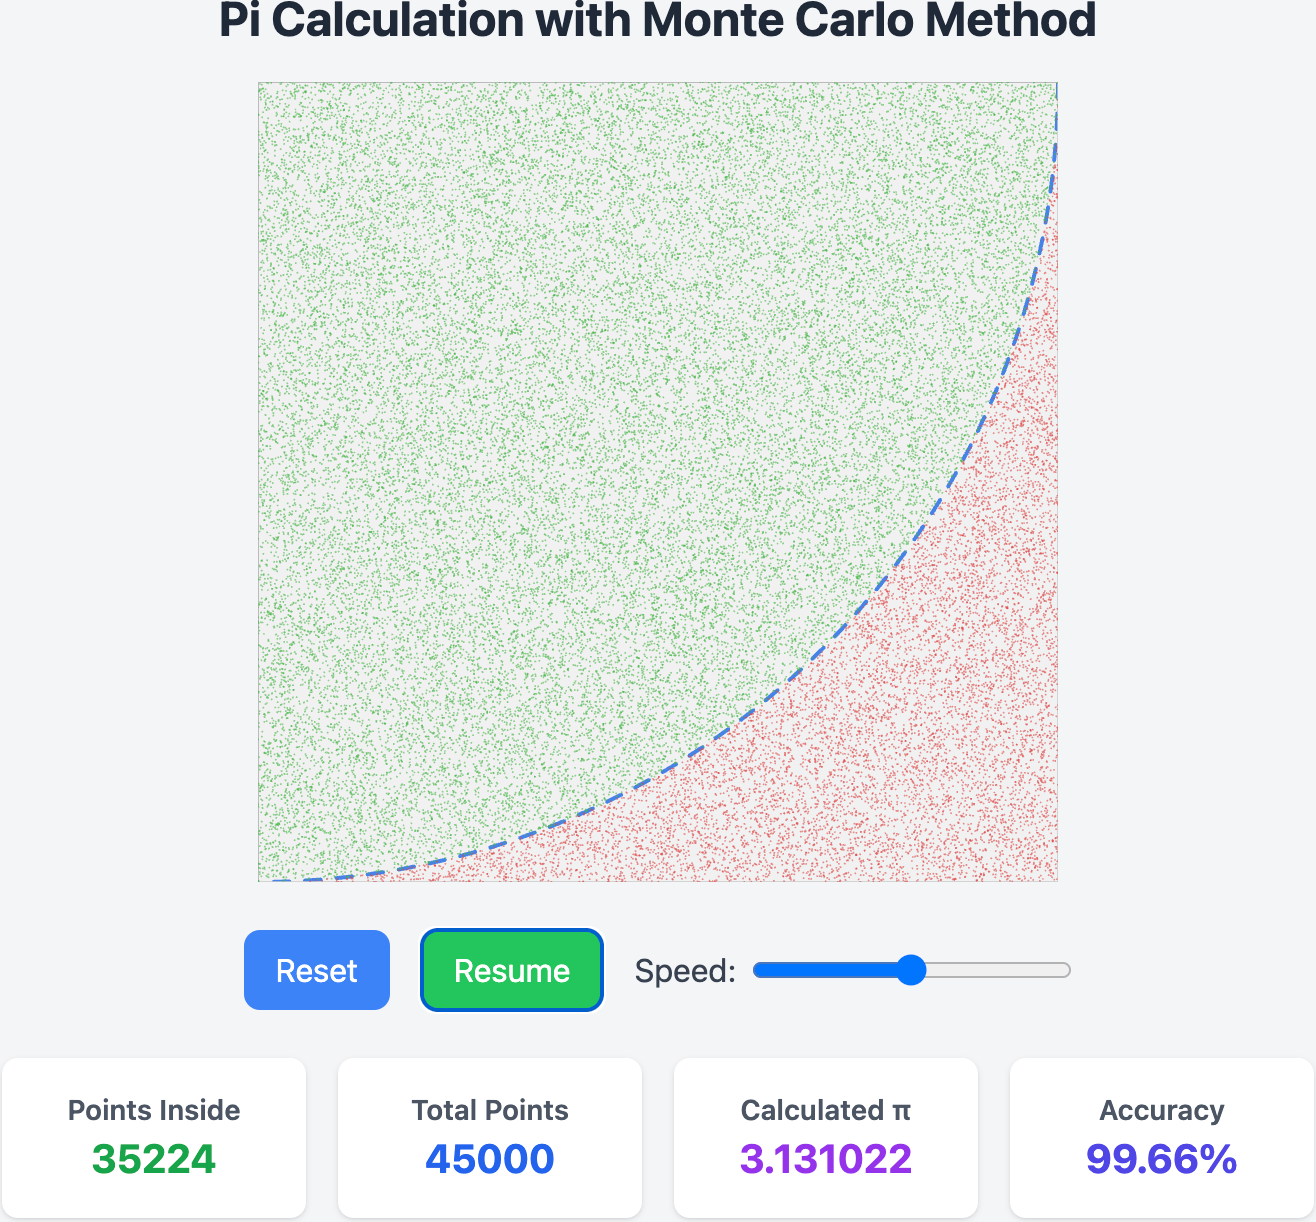
\includegraphics[width=0.4\textwidth]{../programs/pi_calculation/pi_calculation.png}

    \vspace{0.5cm}
    \href{../programs/pi_calculation/pi_calculation.html}{Open Interactive Demo}
    \end{center}
\end{frame}

\section{Analysis: Recurrence and Expectation}
\begin{frame}{Quicksort Recurrence}
  \begin{block}{Expected Comparisons}
    \[
      T(n) \leq n + \frac{1}{n} \sum_{i=1}^n (T(i-1) + T(n-i))
    \]

    Base case: $T(1) = 0$

    Solution: $T(n) = O(n \log n)$
  \end{block}
\end{frame}

\begin{frame}{Slick Analysis: Indicator Variables}
  \begin{itemize}
    \item $Q(A)$: Number of comparisons on input $A$

    \item $X_{ij}$: Indicator for whether elements $i$ and $j$ are compared

    \item $E[Q(A)] = \sum_{i<j} Pr[R_{ij}]$

    \item $Pr[R_{ij}] = \frac{2}{j-i+1}$
  \end{itemize}

  \begin{block}{Visualization}
    \begin{center}
      % Insert comparison probability diagram here
      \begin{tikzpicture}[scale=1, every node/.style={scale=1}]
        % Draw array boxes
        \foreach \i in {1,...,8} {
            \draw (\i,0) rectangle (\i+1,1);
            \node at (\i+0.5,0.5) {\i};
          }
        % Highlight i and j
        \fill[green!20] (2,0) rectangle (3,1);
        \fill[blue!20] (7,0) rectangle (8,1);
        \node at (2.5,0.5) {$i$};
        \node at (7.5,0.5) {$j$};
        % Draw arc between i and j
        \draw[thick,red,->] (2.5,1) .. controls (4.5,2.5) and (6.5,2.5) .. (7.5,1);
        \node[red] at (5,2.7) {Probability $2/(j-i+1)$};
      \end{tikzpicture}
    \end{center}
  \end{block}
\end{frame}

\begin{frame}{Harmonic Numbers in Analysis}
  \begin{block}{Harmonic Number}
    $H_n = \sum_{i=1}^n \frac{1}{i} = \Theta(\log n)$
  \end{block}

  \begin{block}{Summation in Quicksort}
    $E[Q(A)] \leq 2nH_n = O(n \log n)$
  \end{block}
\end{frame}

% Example: Coin Toss Probability
\section{Example: Coin Toss Probability}
\begin{frame}{Coin Toss Example}
  \begin{block}{Experiment}
    John tosses a biased coin (probability $p$ of heads) to decide whether to wear a tie. If heads, tosses a fair coin to pick red or blue tie.
  \end{block}

  \begin{block}{Question}
    What is the probability John wears a red tie on the first day he wears a tie?
  \end{block}

  \begin{center}
    % Insert coin toss diagram here
    \begin{tikzpicture}[level distance=1.5cm,
        level 1/.style={sibling distance=3cm},
        level 2/.style={sibling distance=2cm}]
      \node {Start}
      child {node {Tie ($p$)}
          child {node {Red (0.5)}}
          child {node {Blue (0.5)}}
        }
      child {node {No Tie ($1-p$)}};
    \end{tikzpicture}
  \end{center}
\end{frame}

% Where do random bits come from?
\section{Random Bits in Practice}
\begin{frame}{Where do Random Bits Come From?}
  \begin{itemize}
    \item Hardware random number generators

    \item Pseudo-random number generators (PRNGs)

    \item Physical phenomena (thermal noise, radioactive decay)

    \item In practice, PRNGs are sufficient for most applications
  \end{itemize}
\end{frame}

% Probabilistic Data Structures
\section{Probabilistic Data Structures}

\begin{frame}{What is a Probabilistic Data Structure?}
  \begin{block}{Definition}
    Data structures that use randomization or probabilistic techniques to achieve space or time efficiency, often allowing for small errors (e.g., false positives).
  \end{block}

  \begin{itemize}
    \item Useful for large-scale data, streaming, or approximate answers
    \item Examples: Bloom filter, Count-Min Sketch, HyperLogLog
  \end{itemize}
\end{frame}

\begin{frame}{Bloom Filter: What and Why?}
  \begin{block}{What is a Bloom Filter?}
    A space-efficient, probabilistic data structure for set membership queries.
  \end{block}

  \begin{itemize}
    \item Answers: "Is $x$ in the set?"
    \item May return false positives, but never false negatives
    \item Very compact compared to hash sets
  \end{itemize}
\end{frame}

\begin{frame}{How Does a Bloom Filter Work?}
  \begin{enumerate}
    \item Start with a bit array of $m$ bits, all set to 0

    \item Use $k$ independent hash functions

    \item To add an element, set $k$ bits (one per hash) to 1

    \item To check membership, test if all $k$ bits are 1
  \end{enumerate}
\end{frame}

\begin{frame}{Bloom Filter Example}
  Suppose $m=8$ bits, $k=2$ hash functions, and we insert $\{\text{cat}, \text{dog}\}$.

  \begin{block}{Bit Array After Insertion}
    \[
      \begin{array}{|c|c|c|c|c|c|c|c|}
        \hline
        1 & 0 & 1 & 1 & 0 & 0 & 0 & 1 \\
        \hline
      \end{array}
    \]
  \end{block}

  \begin{itemize}
    \item To check if "cat" is in the set, hash and check the corresponding bits
    \item If all are 1, answer is "possibly in set"; if any is 0, "definitely not in set"
  \end{itemize}
\end{frame}

\begin{frame}{Bloom Filter: Trade-offs}
  \begin{itemize}
    \item \textbf{False positives:} May say "in set" when not

    \item \textbf{No false negatives:} Never says "not in set" if it is

    \item \textbf{Space efficient:} Much smaller than explicit set

    \item \textbf{No deletions:} Standard Bloom filters do not support removing elements
  \end{itemize}
\end{frame}

% References
\begin{frame}[allowframebreaks]{References}
  \printbibliography
\end{frame}

\end{document}
